\chapter[Background]{{\color{red}\fontsize 90 :}Background}
%
\label{ch:background}

\section{First section}\label{ch:forcefeed}

\kant[3]

\section{Second section with a figure}

Figure~\ref{fig:shiptracks} shows some nice patterns.

\begin{figure}
\centering
    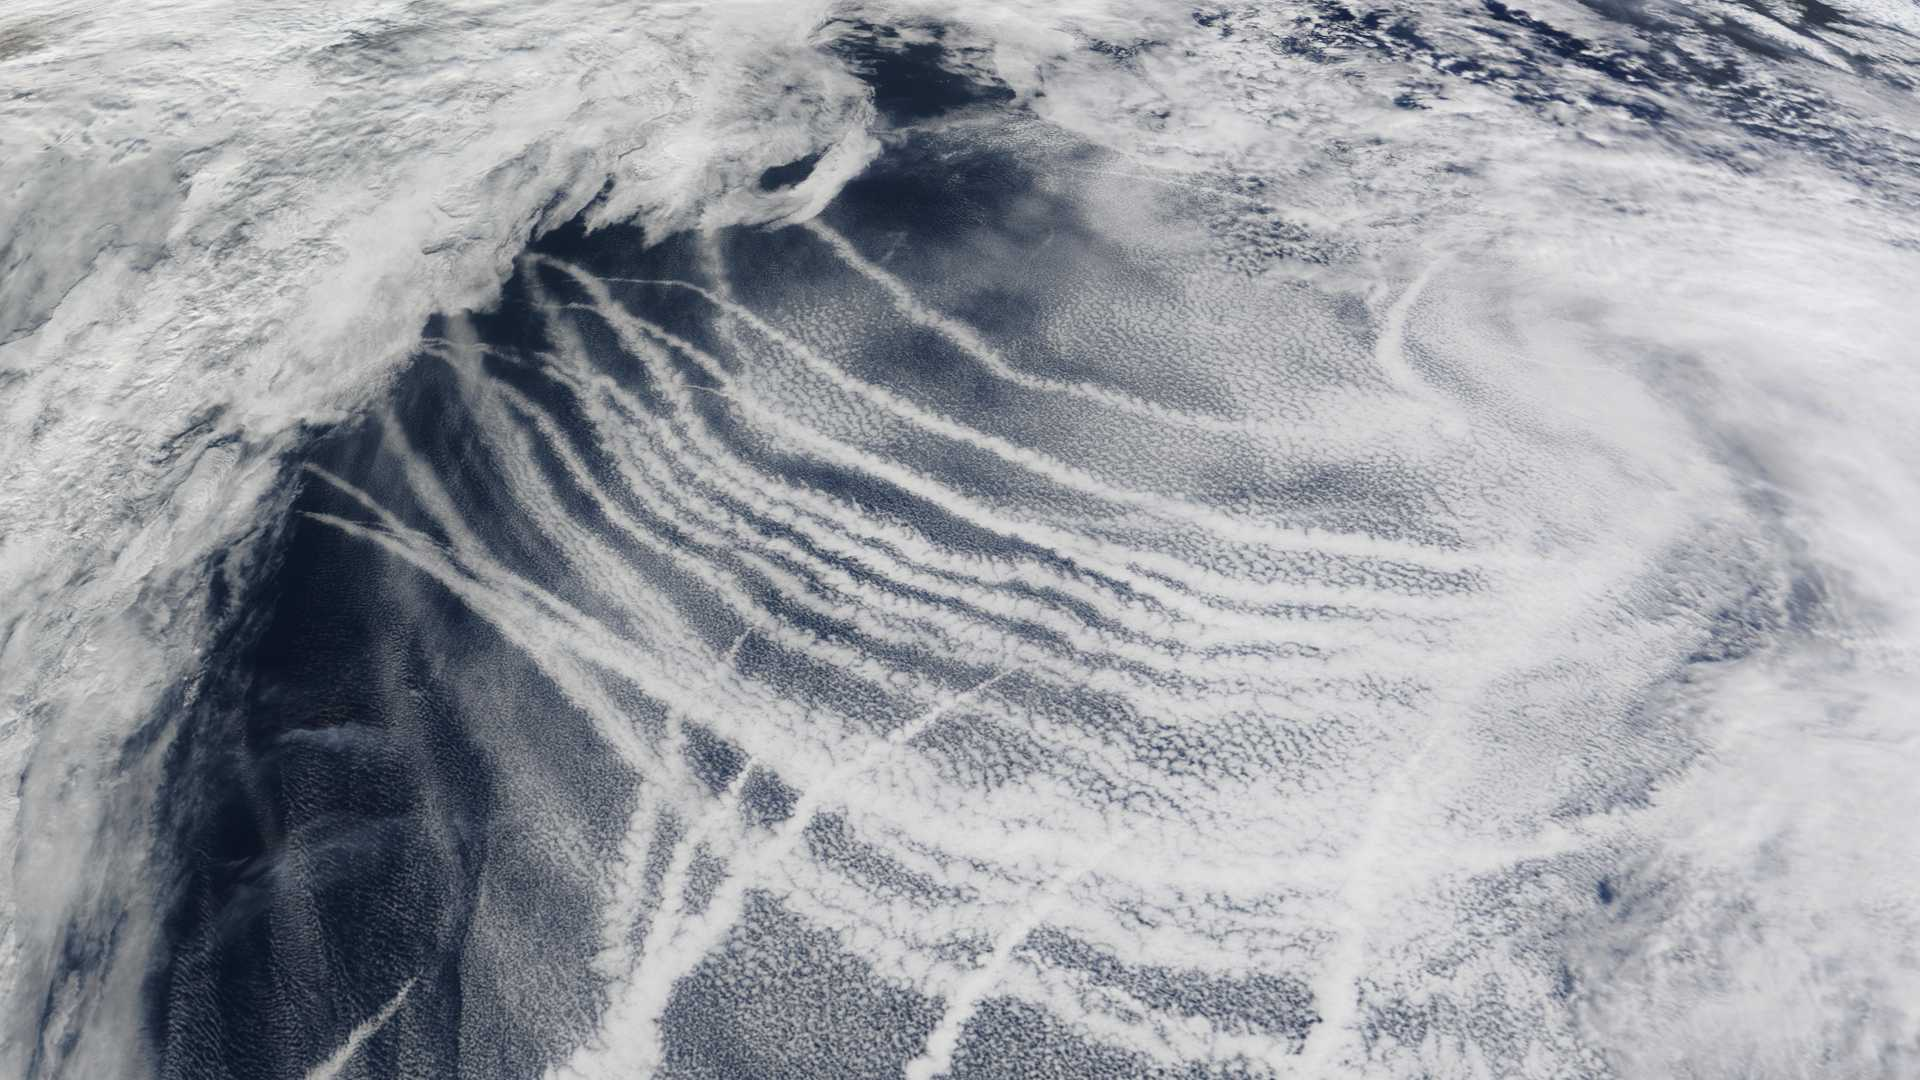
\includegraphics[width=0.65\textwidth]{figures/ship_tracks.jpg}
\caption{\textit{Ship tracks observed by NASA's MODIS instrument on board the Aqua satellite. Figure retrieved from \url{https://svs.gsfc.nasa.gov/3667} October 9, 2019. More information about the instrument is found in Chapter \ref{ch:metode}.}}
\label{fig:shiptracks}
\end{figure}

\subsection{Subsection with reference}
\label{sec:ex:cite}

An example of a citation from a paper~\cite{glasius_composition_2018}.
